% This document is part of the EPRVCalibration project
% Copyright 2019 the authors. All rights reserved.

\documentclass[12pt, letterpaper]{article}
\usepackage{xcolor}
\newcommand{\lz}[1]{\textcolor{orange}{#1}}

\usepackage[ruled,vlined]{algorithm2e}
\usepackage{graphicx}

% typesetting words
\newcommand{\project}[1]{\textsl{#1}}
\newcommand{\acronym}[1]{{\small{#1}}}
\newcommand{\expres}{\project{\acronym{EXPRES}}}
\newcommand{\name}{\project{NameOfThis}}

% margins and page setup, etc
\addtolength{\textheight}{1.00in}
\addtolength{\topmargin}{-0.50in}
\sloppy\sloppypar\raggedbottom\frenchspacing

\begin{document}

\section*{\raggedright%
\name:
A non-parametric, hierarchical model for a laser-comb-calibrated spectrograph}

\noindent
\textbf{Lily~Zhao} (Yale) (Flatiron),
\textbf{David~W~Hogg} (NYU) (MPIA) (Flatiron),
\ldots and others\ldots

\paragraph{Abstract:}
There have been many hardware improvements in polygonal-fiber-fed,
temperature-controlled, laser-frequency-comb or etalon-calibrated,
high-resolution, extreme-precision radial-velocity spectrographs.
Have the calibration methodologies improved to match?
Here are three relevant observations:
The first is that the calibration lines or spots from an etalon or
comb fill the spectral range with dense calibration points.
The second is that the spectrograph lives in a stabilized,
climate-controlled environment, in which the full optical system and
detectors will only vary within a tiny range of configurations or
settings.
The third is that---given this stability--- every calibration image
ever taken is relevant to every science exposure ever taken; there is
no reason to calibrate every exposure independently.
The calibration methodology we propose here---\name---addresses these
three problems by going non-parametric (no more polynomials!) and then
reducing dimensionality with a robust principal-component method.
We demonstrate the success of this method with data from the
\expres\ spectrograph.
We find... [results and so on].

\section{Introduction} 

Why hierarchical?

Why non-parametric?


\section{Method} \label{sec:method}
We are operating on the core idea that the wavelength solution is living in a low-dimensional space, where the degrees of freedom are set by the limited degrees of freedom of the spectrograph hardware.

The way we think about this is the following:
Given an exposure $n$, and order $m$, there is a relationship between
the two-dimensional $(x,m)$-position on the detector and the
wavelength $\lambda$
\begin{equation}
\lambda(x,y,m,n) = f(x,y,m;\theta_{n})
\quad ,
\end{equation}
where $\theta_{n}$ is a big blob of parameters for this exposure.

Taking into account the low-degree of variability a stabilized spectrograph strives for, the calibration of every image can be informed by the calibration of every other image.  To implement this hierarchical model, we use the calibration data themselves to develop a low-dimensional basis for expressing the calibration data.

If the space of all calibration possibilities is in fact $K$-dimensional (where K is a small integer, i.e 2 or 8 or thereabouts thereabouts), and if the calibration variations are so
small that we can linearize, then the function $f(x,y,m;\theta_{n})$ could
be replaced with a tiny model
\begin{equation}
\lambda(x,y,m,n) = g_0(x,y,m) + \sum_{k=1}^K a_{nk}\,g_k(x,y,m)
\quad ,
\end{equation}
where
$g_0(x,y,m)$ is the fiducial or mean or standard calibration of the
spectrograph,
the $a_{nk}$ are scalar amplitudes,
and the $g_k(x,y,m)$ are basis functions expressing the ``directions'' in calibration space that the spectrograph can depart from the
fiducial calibration.
The challenge is to learn these basis functions from the data, and get
the $K$ amplitudes $a_{nk}$ for every exposure $n$.

\subsection{Data} \label{sec:data}
We present results using data from \expres\, the EXtreme PRecison Spectrograph.  \expres\ is an envionmentally stabilized, fiber-fed, $R=137,000$, optical spectrograph (\lz{CJ and RB's papers}).  \expres\ has two different calibration sources, a ThAr lamp and a Menlo Systems laser frequency comb (LFC, e.g. \lz{Wilken+ 2012, Molaro+ 2013, Probst+ 2014, from RB's paper}).  ThAr exposures are taken at the beginning and end of each night.  LFC exposures are interspersed between science exposures every ~15 minutes.  
(Discussion of number of orders covered or number of lines in LFC and/or ThAr?)

\lz{Discussion of line fitting?  Though the current line fitting causes me recurring nightmares.  I should really take the time to look into at least the peak fitting more.}

\expres\ exposures are separated into different ``instrumental epochs," which correspond to changes to the position of the echellogram on the detector, the shape of the instrumental PSF, or the calibration sources (\lz{(worth including table that explicitly defines epochs?)}).  Because significant instrumental changes break the assumption of only low-dimensional variations in the spectrograph hardware, we treat each instrument epoch independently.

\subsection{Hierarchical De-Noising of Calibration Frames} \label{sec:denoising}
% Gotta make this whole section more math-y
% Add variable names for matrix of all lines and exposures, what defines a line, what defines a line measurement, fiducial calibration
let ${exp_n}$ be the set of calibration exposures within an instrument epoch that will be used to construct the basis functions that characterize the potential change in calibration space of each exposure throughout that instrument epoch.  We first identify the full list of lines we can expect to find in a calibration image from this epoch by iterating through all ${exp_n}$ and constructing a list of all unique lines found in these exposures.  A line is uniquely defined by a combination of order, $m$, and ``true" wavelength value, $\lambda$.

For each line, we then find the fitted line center, in pixel space, for that line for each exposure.  If the line is missing from an exposure, we insert a NaN for the line center instead.  Lines that are missing from greater than some percent of exposures are cut.  Exposures that are missing greater than some percent of lines are also cut (\lz{This will miss low signal exposures that suffer most in the first few orders but can recover in later orders; can't decide if this is a feature or a bug}).  This threshold percentage is 50\% for LFC exposures and 30\% for ThAr exposures.

\lz{Discuss separating out sub-epochs due to echellogram shifts from focus motor position changes here if relevant}

Missing lines were replaced with denoised estimates using iterative PCA.  The line center of each missing line are initialized to the mean of the nearest 9 exposures in time.  We then find a fiducial calibration of the spectrograph, which is the mean line center value for each identified line.  We subtract this fiducial calibration from each exposure's measured line centers and run PCA on the difference between the measured and fiducial line center for each exposure.

Using the first K principal components, where K is some small integer like 2, and PCA weights, we reconstruct a de-noised matrix of line centers for each exposure.  Values from this reconstruction is then used to patch missing line centers.  This is done iteratively until the value of missing line centers being patched changes by less than 0.01\% of a pixel.  The last interpolation's principal components and coefficients are returned as well as the fiducial calibration and the de-noised matrix.

\begin{algorithm}
\SetAlgoLined
\While{change in bad pixels $>$ 0.01\%}{
	find fiducial calibration of the spectrograph\;
	determine PCA of line matrix - fiducial calibration\;
	reconstruct line matrix to order K\;
	patch bad pixels with reconstructed line matrix
	}
\caption{Hierarchical De-Noising}
\end{algorithm}

\subsection{Non-Parametric Calibration} \label{sec:nonparam}
We can interpolate the returned PCA coefficients over time to determine the wavelength solution at any given time.  Using the interpolated PCA coefficients and the returned basis vectors, we can construct a de-noised set of line centers for that point in time.  We use a cubic spline to interpolate the PCA coefficients.

Once we have determined line centers for each line, which has an associated known wavelength, we can interpolate the known wavelengths over line centers to any pixel in a given order.  We can either interpolate onto every x pixel, and generate a complete wavelength solution for that order, or interpolate onto the measured line centers of a calibration image and compare the return wavelengths as a validation of our method.  This interpolation is also done using a cubic spline.

\begin{algorithm}
\SetAlgoLined
Inputs: new time, new line centers, new orders\; %command not working for w/e reason
interpolate PCA coefficients to new time\;
reconstruct line matrix for that time\;
\For{each order}{
	identify the new line centers in that order using new orders\;
	Interpolate the info from the line matrix to the new x values\;	
	}
\caption{Non-Parametric Wavelength Solution}
\end{algorithm}

\subsection{Choice Choices} \label{sec:choices}
(Before or after results presented in validation test and ThAr sections?)
\begin{itemize}
	\item Value of K for denoising
	\item Type of interpolation (cubic spline vs nearest neighbor or linear)
	\item Interpolation order (interpolate time and x direction together?  Individually?  Which one first?)
	\item Fitting wavelength as dependent variable?  (Should be line centers, right?)
\end{itemize}

Due to the dispersion intrinsic to echelle spectrographs, the wavelength change between pixels is greater at greater wavelengths.  This means that the function of wavelength given pixel across an order will necessarily be concave down everywhere.  Consequently, linear interpolation of this function will systematically give erroneously low values.


\section{Results} \label{sec:results}
\subsection{Self Tests} \label{sec:test-self}
First, let's have a sanity check.  Using a cubic spline scheme with no smoothing to predict wavelengths for the returned, denoised line center values should return identical values to the assigned true wavelength for each line within machine error.
We do see this, for both ThArs and LFCs: look at the figure.

As an only slightly less silly sanity check, we can also use the constructed PCA basis to predict wavelengths for the measured line centers for an exposure that was included in the set of exposures used to construct the basis.  This interpolation should return identical PCA coefficients for that time.  Differences in wavelengths will arise from a combination of 1) error inherent in measuring line centers and 2) interpolation error of lines to other x positions in the pixel direction.

Difference in denoised x-values to measured ones? (translate into rv shift?)
median and spread in errors in pixel (like 0.006) and RV (like 3.2 m/s?)
Histograms

\subsection{Training and Validation Tests} \label{sec:test-trainNvalid}
A better test is to leave out some percentage of the calibration images while constructing the basis and weights with PCA.  We can then use those basis and weights to predict wavelengths for the calibrations images that were left out and assess how accurate the predictions are.  We will call the used calibration images the ``training set," and the left out exposures the ``validation set."

We chose to use 90\% of available exposures to train the PCA, and leave the remaining 10\% for validation.  Exposures were sorted into either set at random.  This test will finally incorporate testing how well PCA coefficients are interpolated to other times outside of the training set and therefore how well the line centers for each wavelength can be reconstructed at all times.  As before, differences in wavelength will also be drawn from how well line centers are measured and error in interpolating to those measured values.  This second source of error was independently quantified in the second test described in the previous section.

LFC looks good, ThAr is struggling a bit
Difference in denoised x-values to measured ones? (translate into rv shift?)
median and spread in errors in pixel (like 0.006) and RV (like 3.2 m/s?)
Histograms

\subsection{Cross Tests} \label{sec:test-cross}
Similar to the training and validation tests, we can also use one calibration source to construct the PCA basis and weights and the other to test the results.  For example, we can use LFC exposures to construct the wavelength solution, and then use it to predict wavelengths for measured line centers of ThAr wavelengths, which will have assigned true wavelengths.  Likewise, we can use ThAr exposures to predict the wavelengths of LFC lines.  Note that errors in this test will also draw on the difference in quality of the two calibration sources being compared.

LFC predicts ThAr better than ThAr can predict itself.
ThAr predicting LFC is really messing up somehow, and I should figure out what it is (sorry!)

%\subsection{ThAr Stuff?  Or Include it in Previous Subsections?}

\section{Comparisons to Other Methods} \label{sec:comparisons}
Presumably we'll use the training/validation method to compare these?

\subsection{Comparison to Parametric Model}
Previously, the \expres\ pipeline the $\theta_{n}$ comprises the
amplitudes of some 9th-ish-order polynomial in $x$ and $n$, possibly
ignoring $y$?
If so, they (may?) have
\begin{equation}
\lambda(x,y,m,n) = \sum_{i=0}^9\sum_{j=0}^9 c_{nij}\, x^i\,m^j + \mathrm{noise}
\quad ,
\end{equation}
where the $c_{nij}$ are coefficients unique to exposure $n$, and
found for exposure $n$ without regard to any other exposure $n'$.
Further, they may be finding the coefficients $c_{nij}$ that
minimize an objective $Q$ that is something like the L2-norm:
\begin{equation}
Q = ||\lambda(x,y,m,n) - \sum_{i=0}^9\sum_{j=0}^9 c_{nij}\, x^i\,m^j||_2^2
\quad .
\end{equation}

Even in this simple context, where every calibration image $n$ is
treated as its own unique flower, there are improvements to be
made.
For one, the sums should not be from 0 to 9, but instead
\begin{equation}
\sum_{i=0}^9\sum_{j=0}^{9-i}
\quad ,
\end{equation}
because that is the definition of 9th order.
If we are right about this, the fit could be taken to 13th order to obtain
much more expressiveness with (nearly) the same number of fit coefficients.
For another, the objective function could be made soft to permit
catastrophic outliers without destroying the fit.
We might recommend the iteratively reweighted least squares (IRLS).
This would make the fitting more robust.
For yet another, there are rescaling issues for the products $x^i\,m^j$ to
protect the fitting from near-singularities or bad conditioning of the
linear-algebra operators.


\begin{figure}[h]
\centering
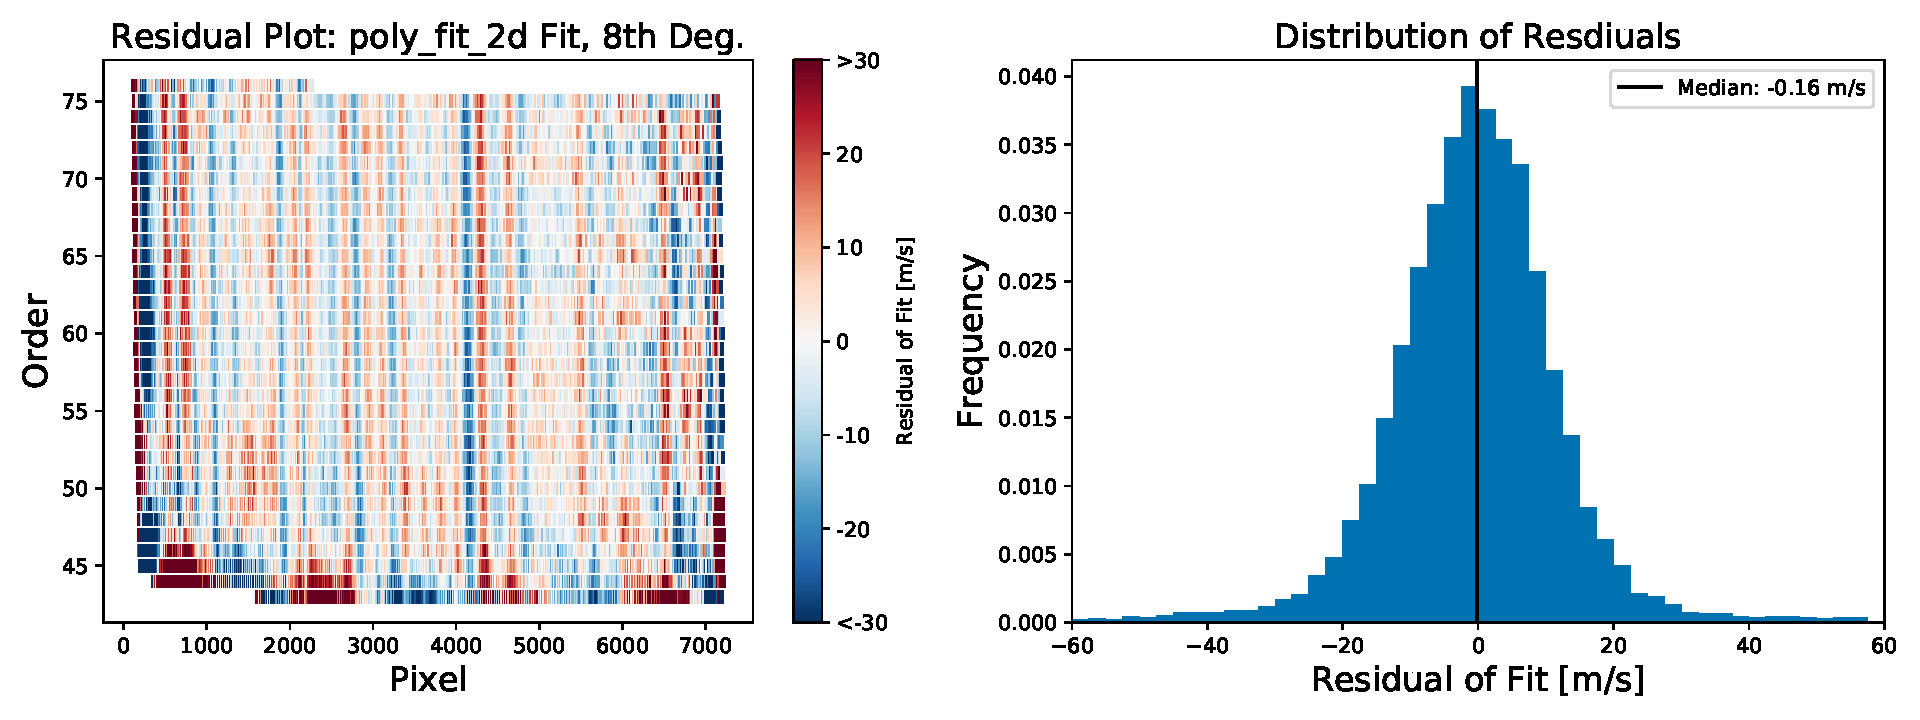
\includegraphics[width=0.9\textwidth]{Figures/polyval2d.pdf}
\caption{}
\label{fig:polyValFit}
\end{figure} 

\begin{figure}[h]
\centering
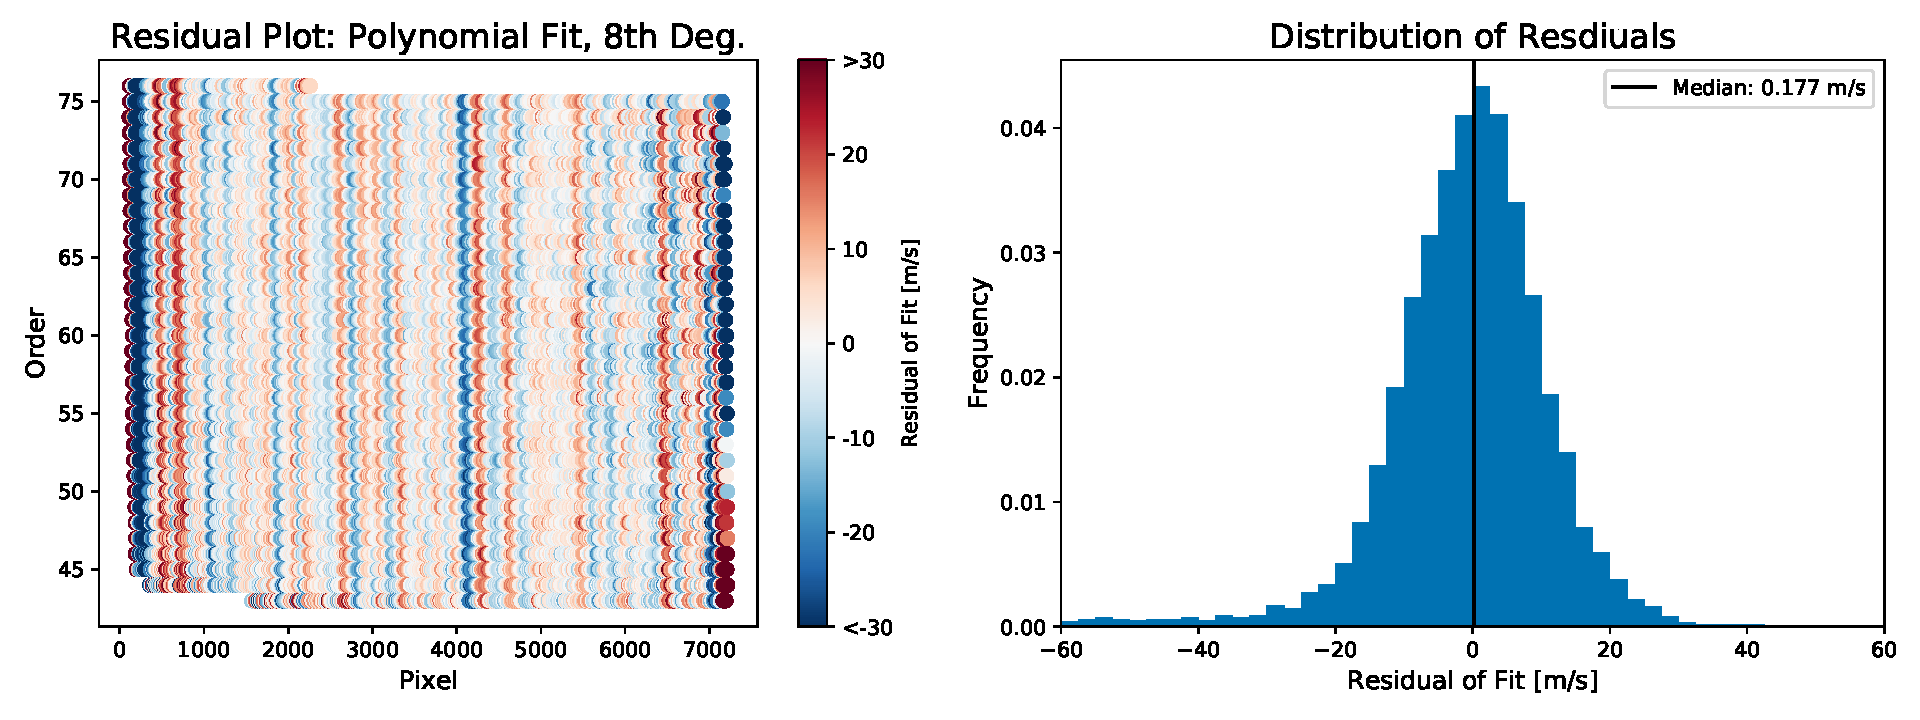
\includegraphics[width=0.9\textwidth]{Figures/designMatrix.pdf}
\caption{}
\label{fig:dsnMFit}
\end{figure} 

\subsection{Comparison to Non-Parametric, Non-Hierarchical Model}

\begin{figure}[h]
\centering
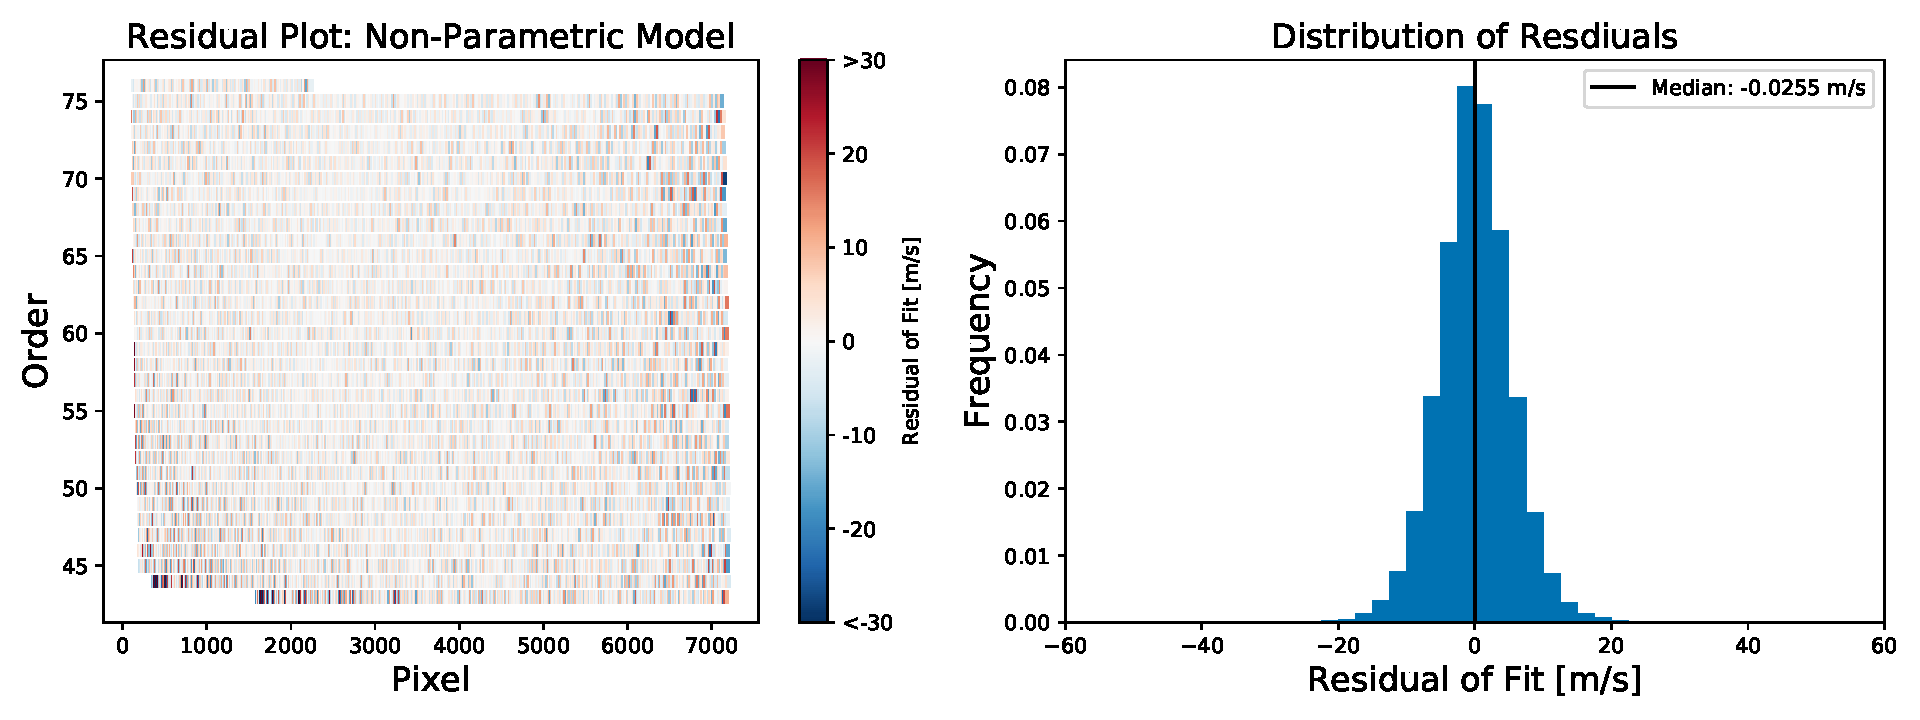
\includegraphics[width=0.9\textwidth]{Figures/noHierc.pdf}
\caption{}
\label{fig:intpFit}
\end{figure} 

\section{Real Data Through to RVs} \label{sec:realdata}

\section{Discussion} \label{sec:discussion}

\end{document}
